\documentclass{report}
\usepackage{enumitem}
\usepackage{clrscode3e}
\usepackage{amsmath}
\usepackage[colorlinks,
            linkcolor=blue,
            anchorcolor=blue,
            citecolor=green,
            pdfauthor=nie_bayes,
            pdfstartpage=1
            ]{hyperref}
\usepackage{graphicx}

\title{Introduction to Algorithms}
\author{Note}

\newcommand{\floor}[1]{\left\lfloor #1 \right\rfloor}

\begin{document}

\maketitle
\tableofcontents

% \textsc{} for definition 
% \textbf{} for leading words of a paragraph

\part{Foundations}
\chapter{The Role of Algorithms in Computing}
\begin{enumerate}[leftmargin=*]
    \item \textsc{Algorithms:} an \emph{algorithm} is any well defined computational procedure that takes some value, or set of values, as \emph{input} and produces some value, or set of values, as \emph{output}. 
    \item \textsc{Data Structure:} a \emph{data structure} is a way to store and organize data in order to facilitate access and modifications. 
    \item \textbf{NP-complete Problems:}
    \begin{itemize}
        \item Although no efficient algorithm for an NP-complete problem has ever been found, nobody has ever proven that an efficient algorithm for one cannot exist. 
        \item If an efficient algorithm exists for any one problem, then efficient algorithms exist for all of them. 
        \item Several NP-complete problems are similar, but not identical, to problems for which we do know of efficient algorithms. Hence a small change to the problem statement can cause a big change to the efficiency of the best known algorithm.
    \end{itemize}
\end{enumerate}

\chapter{Getting Started}
\section{Insertion sort}
\begin{enumerate}[leftmargin=*]
    \item \textbf{Insertion Sort:}
    \begin{itemize}
        \item \textbf{Pseudocode:} 
        \begin{codebox}
        \Procname{$\proc{Insertion-Sort}(A)$} \label{alg:insertion-sort}
        \li \For $j \gets 2$ \To \attrib{A}{length}
            \Do 
        \li     $\id{key} \gets A[j]$ 
        \li     \Comment Insert $A[j]$ into the sorted sequence $A[1 \twodots j-1]$.
        \li     $i \gets j-1$
        \li     \While $i > 0$ and $A[i] > \id{key}$
                \Do
        \li         $A[i+1] \gets A[i]$ 
        \li         $i \gets i-1$
                \End
        \li     $A[i+1] = \id{key}$
            \End
        \end{codebox}
        \item \textsc{In Place}: it rearranges the nunbers within the array \emph{A}, with at most a constant nunber of them stored outside the array at any time. 
        \item \textbf{Loop invariants:}
        \begin{itemize}
            \item Three things about a loop invariant:
            \begin{enumerate}
                \item \textbf{Initialization:} It is true prior to the first iteration of the loop.
                \item \textbf{Maintenance:} If is true before an iteration of the loop, it remains true before the next iteration.
                \item \textbf{Termination:} When the loop terminates, the invariant gives us a useful property that helps show that the algorithms is correct.
            \end{enumerate}
            \item When the loop is a \kw{for} loop, the moment at which we check the loop invariant just prior to the first iteration is immediately after the initial assignment to the loop-counter variable and just before the first test in the loop header.
        \end{itemize}
    \end{itemize}
\end{enumerate}

\section{Analyzing algorithms}
\begin{enumerate}[leftmargin=*]
    \item \textbf{Random-access machine (RAM) model:} 
    \begin{itemize}
        \item In the \emph{RAM} model, instructions are executed one after another, with no concurrent operations.
        \item The \emph{RAM} model constains instructions commonly found in real computers: arithmetic, data movement, and control.
        \item Such computers can compute $2^k$ in one constant-time instruction by shifting the integer 1 by $k$ positions to the left, as long as $k$ is no more than the number of bits in a computer word.
    \end{itemize}
    \item \textbf{Analysis of insertion sort:} \proc{Insertion-Sort} can take different amounts of time to sort two input sequences of the same size depending on how nearly sorted they already are. To analyze it, we need to define the terms "running time" and "size of input" more carefully:
    \begin{itemize}
        \item The best notion for \emph{input size} depends on the problem being studies. 
        \item The \emph{running time} of an algorithm on a particular input is the number of primitive operations or "steps" executed.
    \end{itemize}
    \item \textbf{Worst-case, average-case, and best-case analysis}
    \begin{itemize}
        \item \textbf{Order of growth:} Consider only the leading term of a formula and at the same time ignore the leading term's constant coefficient.
        \item and more \dots
    \end{itemize}
\end{enumerate}

\section{Designing algorithms}
\subsection{The divide-and-conquer approach}
\begin{enumerate}
    \item \textbf{Recursive:} Many useful algorithms are \emph{recursive} in structure: to solve a given problem, they call \emph{themselves} recursively one or more times to deal with closely related subproblems.
    \item \textbf{Divide-and-conquer approach:}
    \begin{enumerate}
        \item \textbf{Divide} the problem into a number of subproblems that are smaller instances of the same problem.
        \item \textbf{Conquer} the subproblems by solving them recursively. If the subproblem sizes are small enough, however, just solve the subproblems in a straightforward manner.
        \item \textbf{Combine} the solutions to the subproblems into the solution for the original problem.
    \end{enumerate}
    \item \textsc{Merge Sort:}
    \begin{itemize}
        \item \textbf{Pseudocode:} 
        \begin{codebox}
        \Procname{$\proc{Merge-Sort}(A,p,r)$} \label{alg:merge-sort}
        \li \If $p < r$
            \Then 
        \li     $q = \floor{(p+r)/2}$
        \li     $\proc{Merge-Sort}(A,p,q)$
        \li     $\proc{Merge-Sort}(A,q+1,r)$
        \li     $\proc{Merge}(A,p,q,r)$
            \End
        \end{codebox}
        \begin{codebox}
        \Procname{$\proc{Merge}(A,p,q,r)$}
        \li $n_1 = q-p+1$
        \li $n_2 = r-q$
        \li let $L[1 \twodots n_1 + 1]$ and $R[1 \twodots n_2 + 1]$ be new arrays 
        \li \For $i = 1 \To n_1$
            \Do 
        \li     $L[i] = A[p+i-1]$
            \End 
        \li \For $j = 1 \To n_2$ 
            \Do 
        \li     $R[j] = A[q+j]$
            \End 
        \li $L[n_1 + 1] = \infty$ 
        \li $R[n_2 + 1] = \infty$
        \li $i = 1$
        \li $j = 1$
        \li \For $k = p \To r$
            \Do
        \li     \If $L[i] \leq R[j]$
                \Then 
        \li         $A[k] = L[i]$
        \li         $i = i+1$
        \li     \Else $A[k] = R[j]$
        \li         $j = j+1$
                \End
            \End
        \end{codebox}
        \item We place at the end of each array a \emph{sentinel} element, which contains a special value $\infty$ that we use to simplify our code.
    \end{itemize}
\end{enumerate}

\subsection{Analyzing divide-and-conquer algorithms}
\begin{enumerate}
    \item \textbf{Recurrence:} When an algorithm contains a recursive call to itself, we can often describe its running time by a \emph{recurrence}, which describes the overall running time on a problem of size $n$ in terms of the running time on smaller inputs.
    \item \textbf{Analyzing the total cost represented by a recurrence:}
    \begin{enumerate}
        \item Construct a \emph{recursion tree}.
        \item Compute the total cost of each level of the tree.
        \item Sum every level's total cost to get the overall total cost.
    \end{enumerate}
    \item \textbf{Recurrence of Merge Sort:} 
    $$
    T(n) = 
    \begin{cases}
        c            & \text{if } n = 1, \\ % You don't necessarily need to line up these two ampersand signs.
        2T(n/2) + cn & \text{if } n > 1.
    \end{cases}
    $$
    \item \textbf{Time complexity:} $T(n) = \Theta(n\lg{n})$
\end{enumerate}

\section{Algorithms}
\begin{enumerate}
    \item \hyperref[alg:insertion-sort]{$\proc{Insertion-Sort}$}
    \item $\proc{Selection-Sort}$
    \begin{codebox}
    \Procname{$\proc{Selection-Sort}(A)$} \label{alg:selection-sort}
    \li $n = \attrib{A}{length}$
    \li \For $j \gets 1 \To n - 1$
        \Do 
    \li     $\id{smallest} \gets j$
    \li     \For $i \gets j + 1 \To n$
            \Do 
    \li         \If $A[i] < A[\id{smallest}]$
                \Then 
    \li             $\id{smallest} = i$
                \End
            \End
    \li     exchange $A[j] \text{ with } A[\id{smallest}]$
        \End
    \end{codebox}
    \item \hyperref[alg:merge-sort]{$\proc{Merge-Sort}$}
    \item $\proc{Bubble-Sort}$ 
    \begin{codebox}
    \Procname{$\proc{Bubble-Sort}(A)$} \label{alg:bubble-sort}
    \li $n = \attrib{A}{length}$
    \li \For $i \gets 1 \To n-1$
        \Do 
    \li     \For $j \gets n \Downto i+1$
            \Do 
    \li         \If $A[j] < A[j-1]$
                \Then 
    \li             exchange $A[j] \text{ with } A[j-1]$
                \End
            \End
        \End
    \end{codebox}
    \item $\proc{Linear-Search}$
    \begin{codebox}
    \Procname{$\proc{Linear-Search}(A, \nu)$} \label{alg:linear-search}
    \li $n = \attrib{A}{length}$
    \li \For $i \gets 1 \To n$
        \Do 
    \li     \If $\nu \isequal A[i]$
            \Then 
    \li         \Return $i$
            \End
        \End
    \li \Return \const{nil}
    \end{codebox}
    \item $\proc{Binary-Search}$
    \begin{codebox}
    \Procname{$\proc{Binary-Search}(A, \nu, low, high)$}
    \li \If $low > high$
        \Then 
    \li     \Return \const{nil}
        \End
    \li $mid = \floor{(low+high)/2}$
    \li \If $\nu \isequal A[mid]$
        \Then 
    \li     \Return \id{mid}
    \li \ElseIf $\nu > A[mid]$
        \Then 
    \li     \Return $\proc{Binary-Search}(A, \nu, mid+1, high)$
    \li \Else \Return $\proc{Binary-Search}(A, \nu, low, mid-1)$
        \End
    \end{codebox}
    \item $\proc{Inversions}$
    \begin{codebox}
    \Procname{$\proc{Count-Inversions}(A,p,r)$} \label{alg:count-inversions}
    \li $\id{inversions} \gets 0$
    \li \If $p < r$
        \Then 
    \li     $q = \floor{(p+r)/2}$
    \li     $\id{inversions} = \id{inverions} + \proc{Count-Inversions}(A,p,q)$
    \li     $\id{inversions} = \id{inverions} + \proc{Count-Inversions}(A,q+1,r)$
    \li     $\id{inversions} = \id{inverions} + \proc{Merge-Inversions}(A,p,q,r)$
        \End
    \li \Return \id{inversions}
    \end{codebox}
    \begin{codebox}
    \Procname{$\proc{Merge-Inversions}(A,p,q,r)$}
    \li $n_1 = q-p+1$
    \li $n_2 = r-q$
    \li let $L[1 \twodots n_1 + 1]$ and $R[1 \twodots n_2 + 1]$ be new arrays 
    \li \For $i = 1 \To n_1$
        \Do 
    \li     $L[i] = A[p+i-1]$
        \End 
    \li \For $j = 1 \To n_2$ 
        \Do 
    \li     $R[j] = A[q+j]$
        \End 
    \li $L[n_1 + 1] = \infty$ 
    \li $R[n_2 + 1] = \infty$
    \li $i = 1$
    \li $j = 1$
    \li $\id{inversions} \gets 0$
    \li $\id{counted} \gets \const{false}$
    \li \For $k = p \To r$
        \Do
    \li     \If $\id{counted} \isequal \const{false} \text{ and } R[j] < L[i]$
            \Then
    \li         $\id{inversions} = \id{inverions} + n_1 - i + 1$
    \li         $\id{counted} \gets \const{true}$
            \End
    \li     \If $L[i] \leq R[j]$
            \Then 
    \li         $A[k] = L[i]$
    \li         $i = i+1$
    \li     \Else $A[k] = R[j]$
    \li         $j = j+1$
    \li         $\id{counted} = \const{false}$
            \End
        \End
    \li \Return \id{inversions}
    \end{codebox}
\end{enumerate}

\subsection{Summary of sorting algorithms}
\begin{figure}[ht]
    \centering
    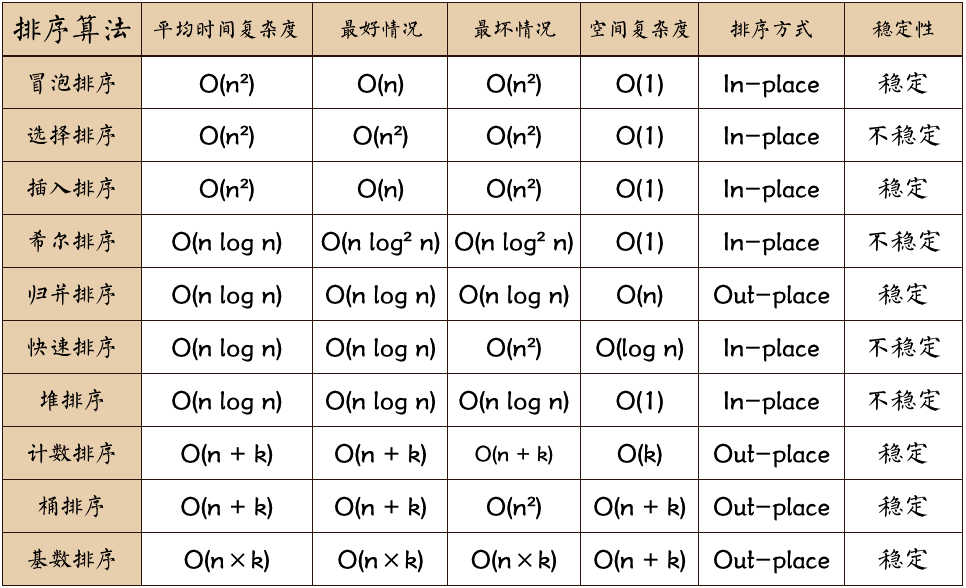
\includegraphics[scale=0.3]{figures/sort_algo_summary.png}
    \caption{Summary of sorting algorithms}
    \label{fig:sort_algo_summary}
\end{figure}

\chapter{Growth of Functions}

\section{Asymptotic notation}

\section{Standard notations and common functions}

\section{Algorithms}

\end{document}